\chapter{Evaluation of t-SNE for H$\alpha$ Emission Candidate Selection}

\section{Introduction to t-SNE}

t-distributed stochastic neighbour embedding, or t-SNE is a dimensionality reduction technique \cite{van2008visualizing} that can be used to map higher dimensional data to a two dimensional plane. This t-SNE map can the be used to cluster and classify similar data points into groups and classes using clustering techniques such as DBSCAN. Often, similar objects will be in close proximity to each other in the lower dimensional space. However, this is not guaranteed. In particular, this similarity measure may not be sensitive to morphological differences in the spectra. Thus, the use of t-SNE must be carefully evaluated if it is to be used as an H$\alpha$ emission candidate selection subroutine as proposed by work such as Traven et al. \cite{traven2017galah}.

Thus DR3 spectra of high dimensionality, can be mapped to a two dimensional representation in order to overcome the curse of dimensionality. If it can be assumed that relevant features in the higher dimensional representation that are common to H$\alpha$ emission candidates are preserved during the mapping from higher dimensions to two dimensions, then this fact can be used to segment H$\alpha$ emission candidates into a distinct class. This class can then be used as a starting point for further analysis using the DTW pipeline demonstrated in chapter 4. 

t-SNE has been used successfully in the past to separate and segment a subset of H$\alpha$ emission candidates in the GALAH survey \cite{traven2017galah}. This study isolated 215 H$\alpha$ and H$\beta$ candidates from a prior GALAH data release of approximately 300,000 spectra. 

However, the preservation of features from high dimensions to two dimensions such that H$\alpha$ emission candidates can be meaningfully separated from normal or average spectra is not guaranteed. The pipeline for P Cygni and inverse P Cygni detection presented in chapter 4 relies on a meaningful and confident selection of H$\alpha$ emission candidates from the GALAH survey prior to the application of DTW and clustering. In subsequent sections, this chapter will demonstrate that t-SNE may not be a sufficiently robust technique to serve as the H$\alpha$ emission candidate selection step that is critical for the DTW based framework presented in chapter 4.

\subsection{Mathematical foundations of t-SNE}

This section presents a brief mathematical introduction to t-SNE adapted from Traven et al. \cite{traven2017galah}. A more detailed discussion is found in Van der Maaten and Hinton \cite{van2008visualizing}. 

Consider $N$ spectra where each spectrum is a higher dimensional object $x_i$. The low dimensional representation of this data is achieved by the optimal positioning of data points in the lower dimensional projection map. In order to achieve this, the t-SNE process defines a similarity between data points in the original higher dimensional space $X$ and in the lower dimensional project space, (2-dimensional for the purpose of this work) $Y$. These are described by the symmetric joint-
probability distributions $P$ and $Q$, respectively

The pairwise similarity between data points $x_i$ and $x_j$ is modeled by the probability that one data point would pick another data point as it's neighbour. This depends on the probability density under a Gaussian in space $X$ while a Student's t-distribution is used in space $Y$. t-SNE first computes probabilities $p_{ij}$ that are proportional to the similarity of spectra $x_i$ and $x_j$ as follows,


For $i$ $\neq$ $j$,

\begin{equation}
p_{j\mid i}={\frac {\exp(-\lVert \mathbf {x} _{i}-\mathbf {x} _{j}\rVert ^{2}/2\sigma _{i}^{2})}{\sum _{k\neq i}\exp(-\lVert \mathbf {x} _{i}-\mathbf {x} _{k}\rVert ^{2}/2\sigma _{i}^{2})}}
\end{equation}

Note that $p_{i\mid i}=0$ and $\sum _{j}p_{j\mid i}=1$ for all $i$. Now define,

\begin{equation}
    p_{ij}={\frac {p_{j\mid i}+p_{i\mid j}}{2N}}
\end{equation}

and note that $p_i_j=p_j_i$, $p_i_i=0$ and $\sum _{ij} p_i_j=1$

The bandwidth of the Gaussian distribution $\sigma_i$ is set such that the perplexity of the conditional distribution equals a predefined perplexity. This perplexity is a user defined quantity and is considered a hyper-parameter of this method. This implies that the bandwidth is adapted to the density of the data, Smaller values of $\sigma_i$ are thus used in denser parts of the data space $X$. 

Next, t-SNE will attempt to learn a lower dimensional map with objects $y_i$ in $Y$ that reflect the similarities $p_i_j$ computed above as well as possible. The process measures similarities $q_i_j$ between two points $y_i$ and $y_j$ using a similar approach. 

For $i$ $\neq$ $j$,

\begin{equation}
    q_{ij}={\frac {(1+\lVert \mathbf {y} _{i}-\mathbf {y} _{j}\rVert ^{2})^{-1}}{\sum _{k}\sum _{l\neq k}(1+\lVert \mathbf {y} _{k}-\mathbf {y} _{l}\rVert ^{2})^{-1}}}
\end{equation}

Here $q_i_i=0$ and the t-distribution with one degree of freedom is used to measure similarities between the lower dimensional points. Thus, dissimilar objects will be projected further apart on the map $Y$.

In order to determine the locations $y_i$ on the map $Y$, the non symmetric Kullback–Leibler divergence shown below is minimized using gradient descent. The result of this optimization scheme is a lower dimensional map of the spectral data.

\begin{equation}
    \mathrm {KL} \left(P\parallel Q\right)=\sum _{i\neq j}p_{ij}\log {\frac {p_{ij}}{q_{ij}}}
\end{equation}

This research uses the t-SNE implementation from the popular Python package \texttt{scikit-learn} to generate all t-SNE mappings and results. While other implementations such as multi-core t-SNE exist \cite{Ulyanov2016}, the performance gains of using processor optimised versions of t-SNE over the \texttt{scikit-learn} implementation are modest in this context.

\section{Application of t-SNE to classify H$\alpha$ emission candidates}

This research used an identical approach to Traven et al. on DR3 data to attempt to isolate, cluster and classify potential H$\alpha$ candidates. Such candidates can then be subjected to the pipeline proposed in chapter 4. The first step of this approach involves using t-SNE to dimensionally reduce spectra to a 2-dimensional t-SNE map. The spectra were masked to select the H$\alpha$ region only \cite{traven2017galah}. The perplexity parameter was set to 30 as this provided reasonable separation of classes in Traven et al.

\begin{figure}[h]
\centering
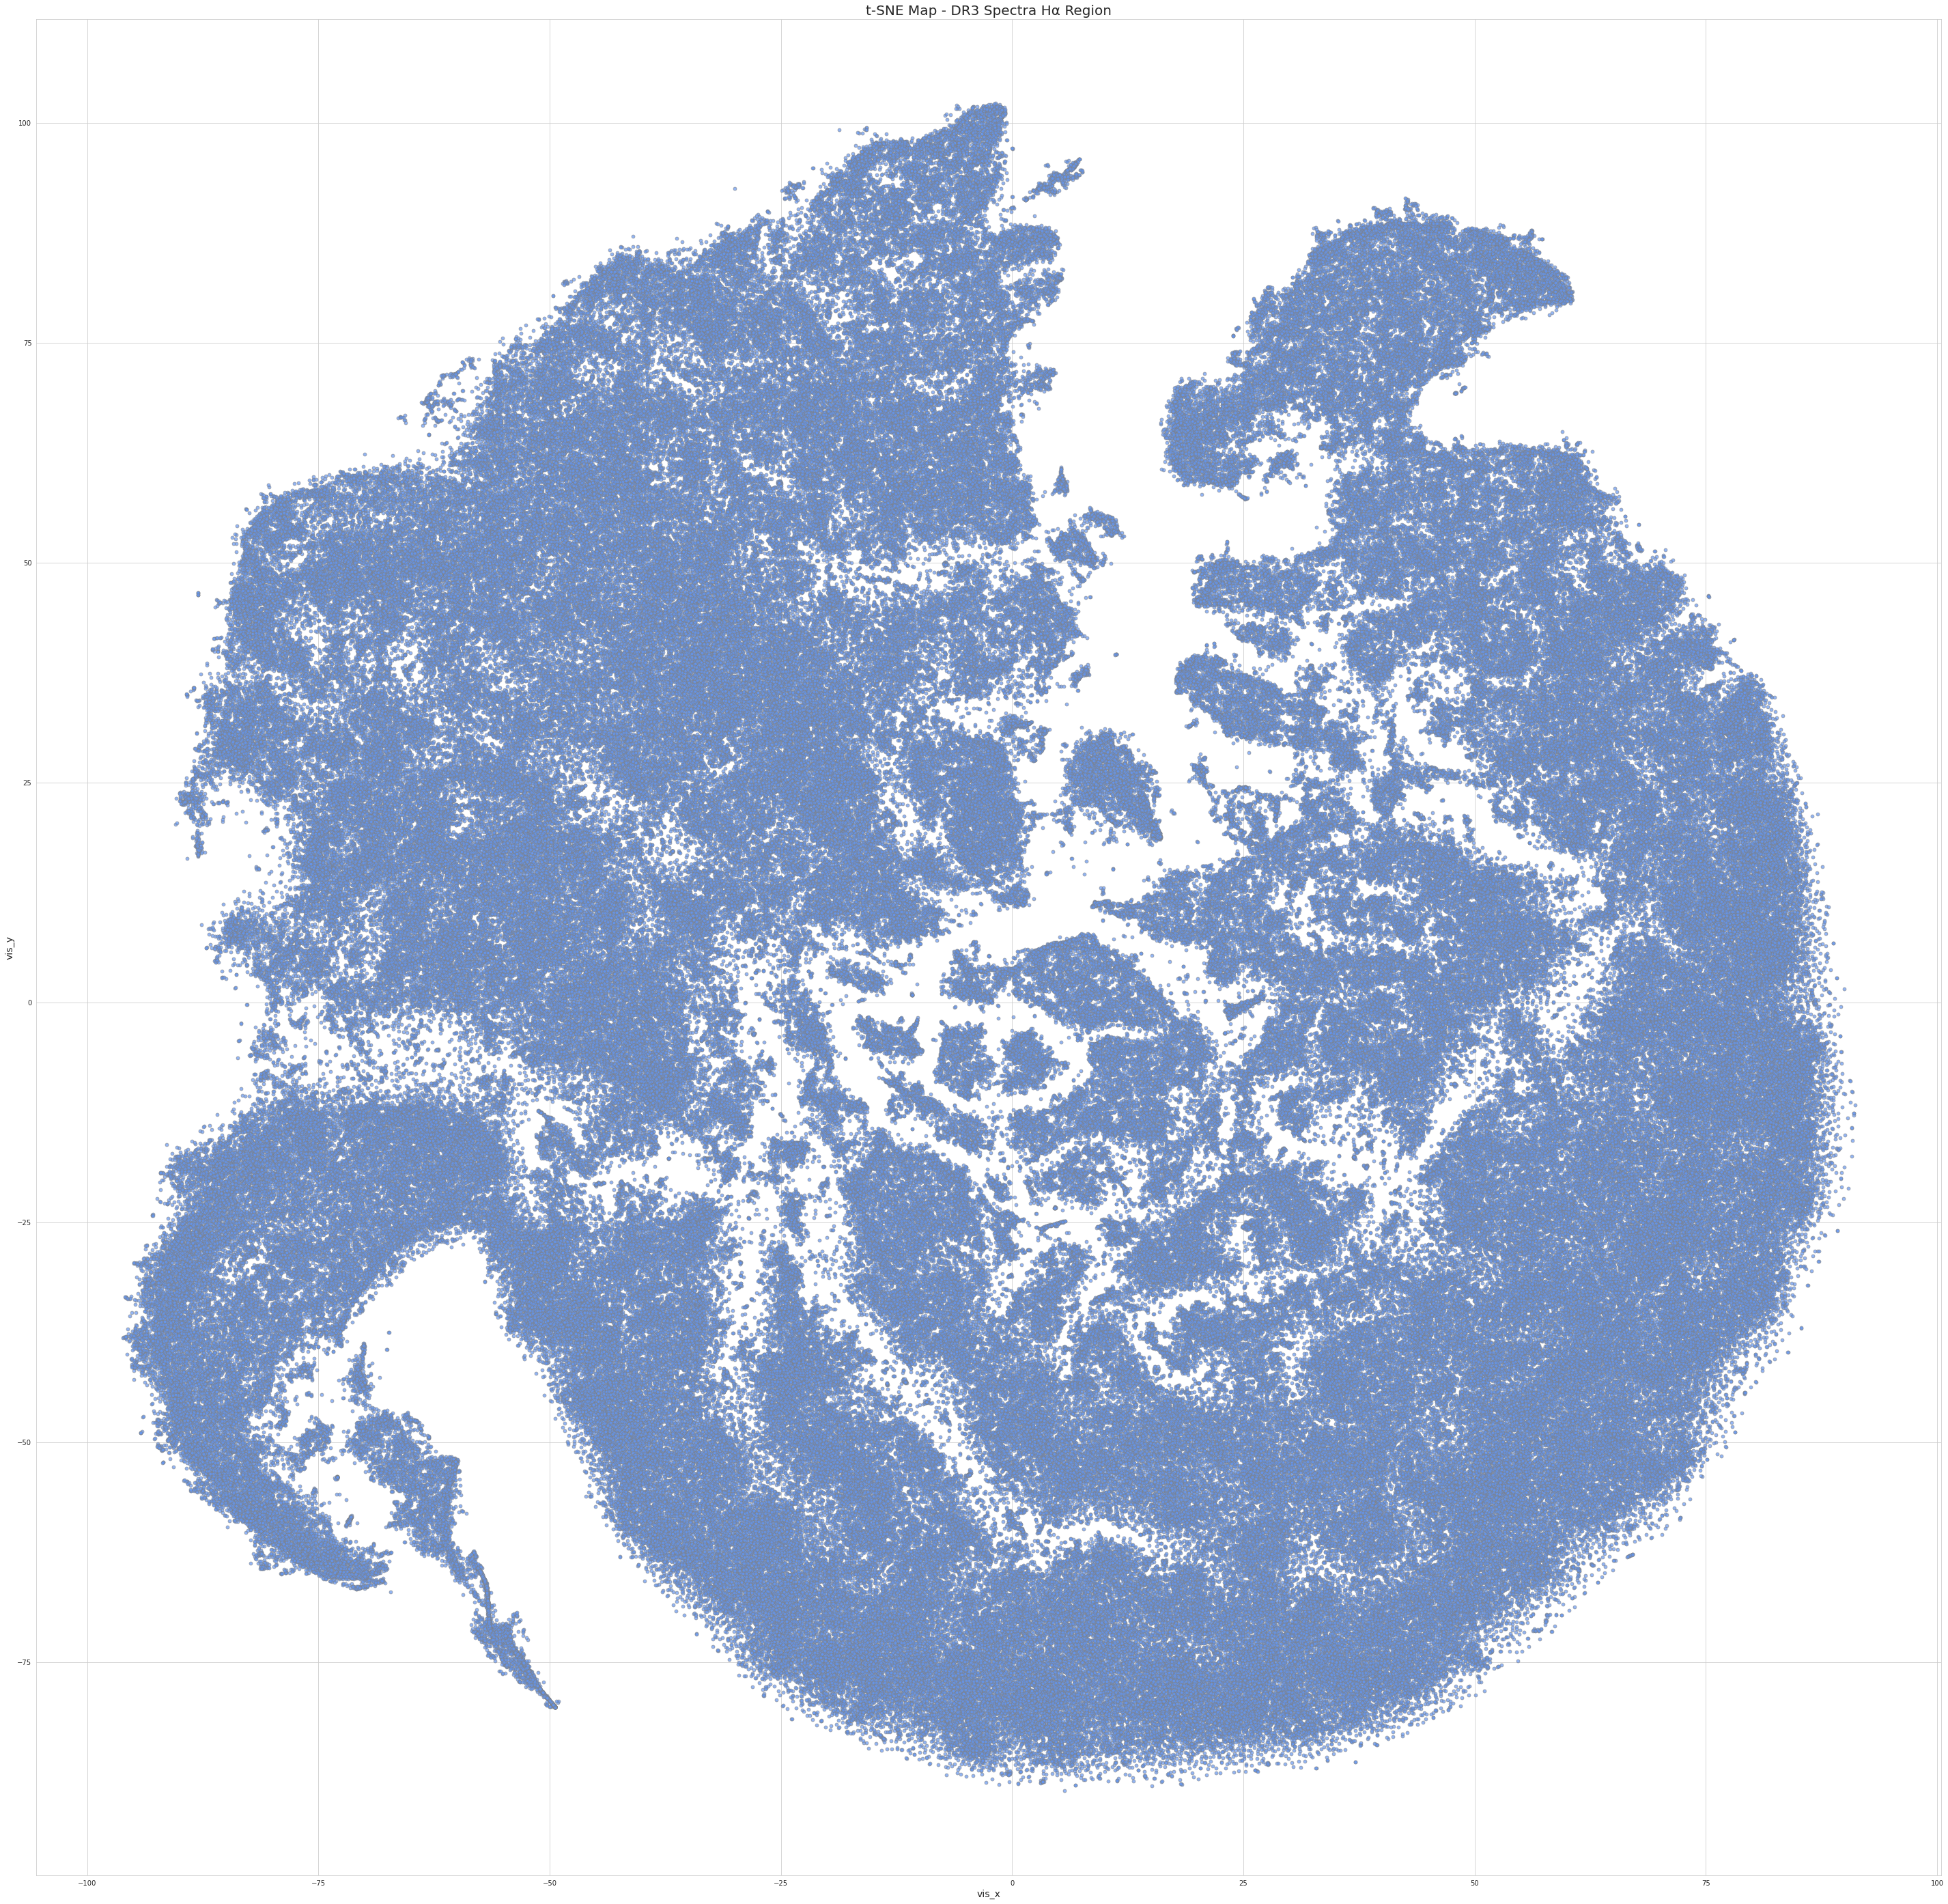
\includegraphics[scale=0.12]{figures/t-sne halpha masked.png}
\caption{t-SNE map for all spectra in DR3. Each point is a 2-dimensional representation of a spectrum. Note that only the region around H$\alpha$ of each spectrum was used to generate this map. The $x$ and $y$ axes contain physically meaningless quantities.}
\end{figure}

\begin{figure}[t]
\centering
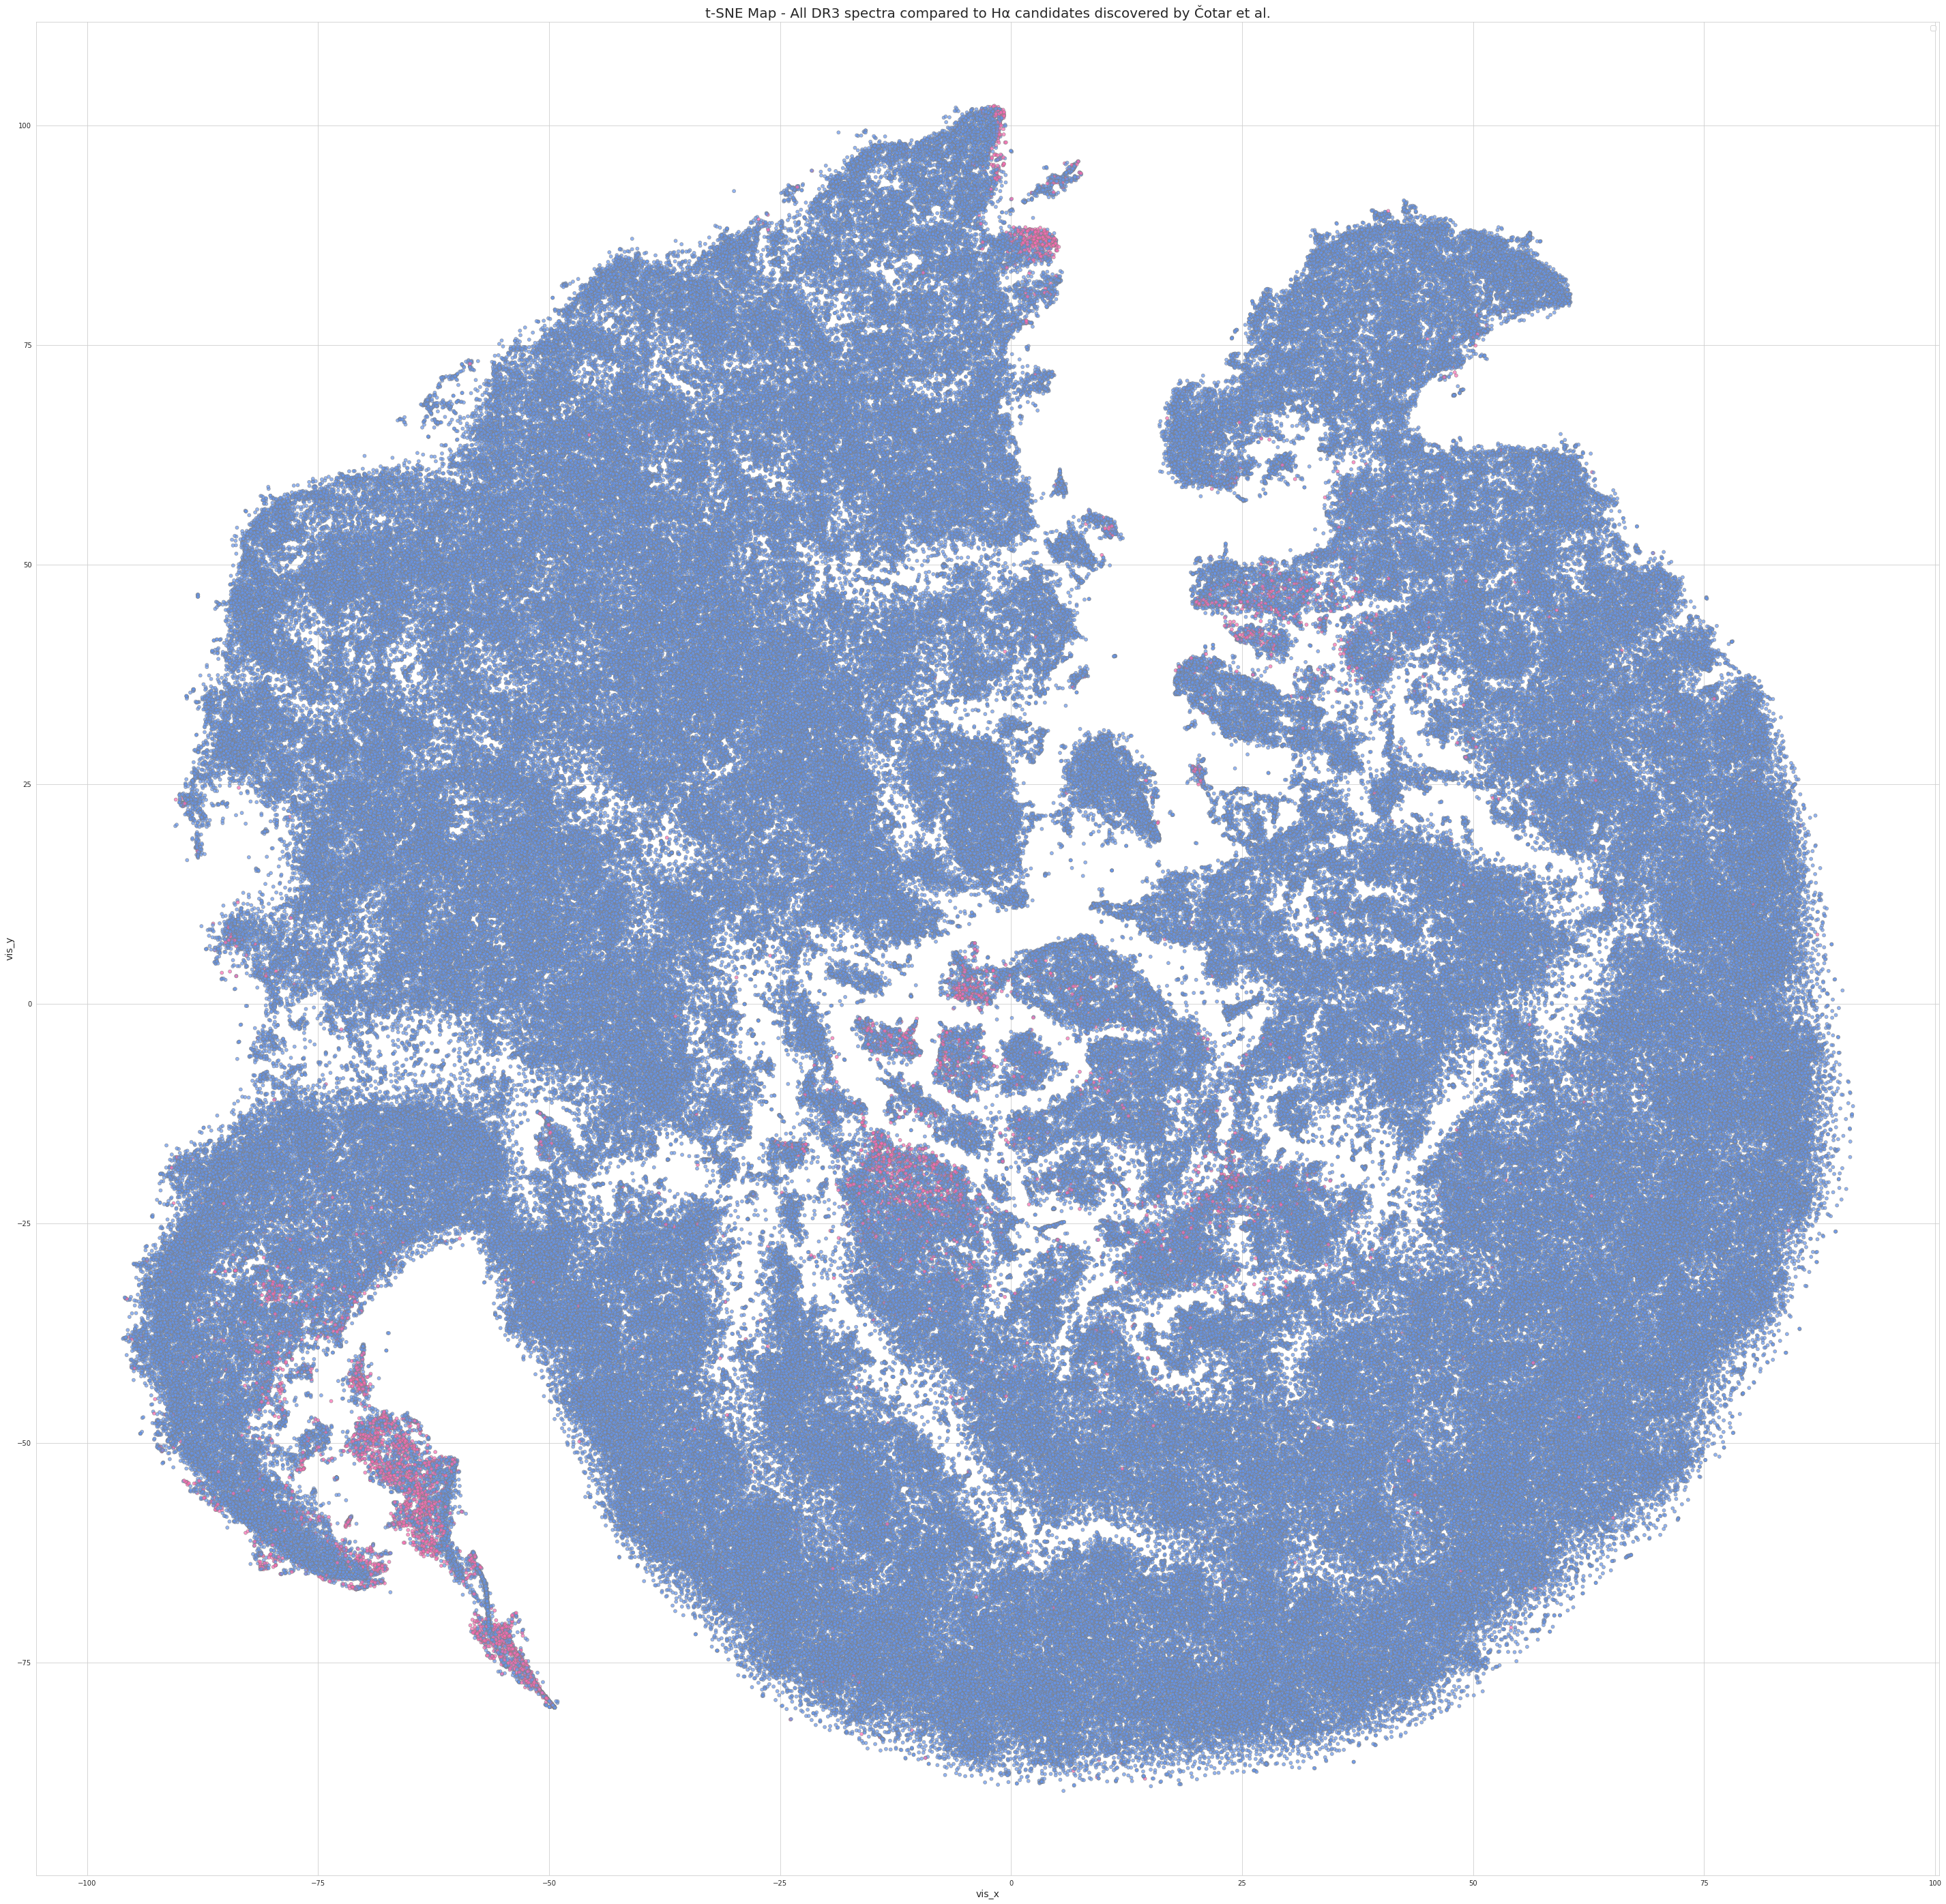
\includegraphics[scale=0.12]{figures/t-sne halpha masked with cotar.png}
\caption{t-SNE map for all spectra in DR3 with H$\alpha$ candidates identified by Čotar et al. tagged in pink.}
\end{figure}

In order to validate if the t-SNE plot can adequately separate H$\alpha$ candidates, the validated H$\alpha$ candidates discovered by Čotar et al. \cite{vcotar2021galah} were marked on the same map by using the object IDs. These 7786 spectra are marked in pink in figure 5.2. While a portion of these candidates are clustered in the bottom left quadrant of the map, the other spectra remain scattered across the map with no obvious meaningful cluster that can be separated out of the t-SNE map. 

The current research followed the distance based clustering method used by Traven et al. but could not meaningfully separate the 7786 H$\alpha$ identified by Čotar et al. using this method. Further details of this process and results are provided in the appendix.

\section{Application of t-SNE to classify P Cygni and inverse P Cygni spectra}

The conclusion that can be drawn from the results in section 5.2 is that H$\alpha$ canididates of the order of thousands of spectra cannot be meaningfully separated by the application of clustering methods on the t-SNE plot generated by the method outlined in Traven et al. Other permutations of hyper parameters such as preplexity may be able to yield better results. However this work based their t-SNE routines on Traven et al. and thus this approach did not yield a significant sample that could be fed into the DTW based scheme proposed in chapter 4. 

This research also examined a proposal made by Traven et al. that a second application of t-SNE on H$\alpha$ candidates can cluster and classify P Cygni and inverse P Cygni candidates. In order to evaluate this approach, this research relied on the H$\alpha$ emission candidates identified by Čotar et al. The proposed approach was as follows,

\begin{enumerate}
    \item Generate a t-SNE map of the H$\alpha$ candidates identified by Čotar et al. using the hyper parameters suggested by Traven et al.
    \item Using object IDs, map the ten clusters identified by the methodology proposed in chapter 4 onto this map
    \item Validate if t-SNE is able to meaningfully separate the P Cygni and inverse P Cygni spectra identified by the methodology proposed in chapter 4
\end{enumerate}

\begin{figure}[h]
\centering
\includegraphics[scale=0.12]{figures/t-sne cotar et al.png}
\caption{t-SNE map for H$\alpha$ candidates identified by Čotar et al. in DR3}
\end{figure}

Note that the representation is significantly simpler compared to the prior application of t-SNE to DR3. The ten clustered identified by the DTW based methodology outlined in chapter 4 yields the following map.

\begin{figure}[t]
\centering
\includegraphics[scale=0.16]{figures/t-sne colored by dtw.png}
\caption{t-SNE map for H$\alpha$ candidates identified by Čotar et al. labelled based on DTW based clustering.}
\end{figure}

Here the P Cygni candidates are represented by cluster 8 and by the colour lime-green while the inverse P Cygni spectra are represented by cluster 9 and the colour teal. Note that cluster 8 appears in two physically separate regions of the t-SNE map and as does cluster 9. Thus it is clear that the application of t-SNE on the H$\alpha$ candidates identified by Čotar et al. does not meaningfully separate P Cygni and inverse P Cygni spectra into distinct regions of the t-SNE map.